\documentclass[aps,prd,twocolumn,superscriptaddress,preprintnumbers,floatfix,nofootinbib]{revtex4-2}

\usepackage{showyourwork}
\usepackage{amsfonts,amssymb,amsmath}
\usepackage[nolist,nohyperlinks]{acronym}

\newcommand*{\mi}[1]{\textsf{\color{magenta} [\textbf{MAX:} #1]}}
\newcommand*{\wf}[1]{\textsf{\color{cyan} [\textbf{WILL:} #1]}}

\begin{document}

\title{Constraining gravitational wave amplitude birefringence with GWTC-3}

\author{Thomas C. K. Ng}
\email{thomas.ng@link.cuhk.edu.hk}
\affiliation{Department of Physics, The Chinese University of Hong Kong, Shatin, Hong Kong}

\author{Maximiliano Isi}
\email{misi@flatironinstitute.org}
\affiliation{Center for Computational Astrophysics, Flatiron Institute, 162 5th Ave, New York, NY 10010, United States}

\author{Kaze W. K. Wong}
\email{kwong@flatironinstitute.org}
\affiliation{Center for Computational Astrophysics, Flatiron Institute, 162 5th Ave, New York, NY 10010, United States}

\author{Will M. Farr}
\email{wfarr@flatironinstitute.org}
\affiliation{Center for Computational Astrophysics, Flatiron Institute, 162 5th Ave, New York, NY 10010, United States}
\affiliation{Department of Physics and Astronomy, Stony Brook University, Stony Brook NY 11794, United States}

\date{\today}

\begin{abstract}
    The propagation of gravitational waves can reveal fundamental features of the structure of spacetime.
    For instance, differences in the propagation of gravitational-wave polarizations would be a smoking gun for parity violations in the gravitational sector, as expected from birefringent theories like Chern-Simons gravity.
    Here we look for evidence of amplitude birefringence in the latest LIGO-Virgo catalog (GWTC-3) through the use of birefringent templates inspired by dynamical Chern-Simons gravity.
    From 71 binary-black-hole signals, we obtain the most precise constraints on amplitude birefringence yet, an order of magnitude more stringent than previous results.
\end{abstract}

\maketitle

\begin{acronym}
\acro{GW}{gravitational wave}
\acro{GR}{general relativity}
\acro{CBC}{compact-binary coalescence}
\acro{BH}{black hole}
\acro{BBH}{binary black hole}
\acro{LVK}{LIGO-Virgo-KAGRA Collaboration}
\acro{PE}{parameter estimation}
\acro{FAR}{false-alarm rate}
\acro{GWOSC}{the Gravitational Wave Open Science Center}
\end{acronym}

\section{Introduction}
\label{sec:Introduction}
% Motivation
\Ac{GW} detections by the \ac{LVK} \citep{LIGO, Virgo, KAGRA} are now routinely used to test various aspects of Einstein's theory of \ac{GR} \citep{LIGOScientific:2016lio,LIGOScientific:2018dkp,LIGOScientific:2021sio}.
Among those, measurements of the basic properties of \acp{GW}, like their speed and polarization, can directly probe the fundamental symmetries of the underlying theory of gravity \citep{Will:2018bme}.
For instance, unequal propagation of \ac{GW} polarization eigenstates would reveal that spacetime is birefringent, a smoking gun for parity-odd theories like Chern-Simons gravity \citep{Jackiw:2003pm,Alexander:2009tp,Sopuerta:2009iy}.
Here we constrain the magnitude of possible amplitude birefringence using \ac{BBH} signals from the latest \ac{LVK} catalog, GWTC-3 \citep{GWTC-3}.

% Previous studies
Previous studies have constrained amplitude birefringence by performing different statistical analyses.
\citet{Yamada_2020} and \citet{Wang_2021} both performed \ac{PE} on the events in the first \ac{GW} transient catalog \citep{GWTC-1}, GWTC-1, using birefringent templates.
\citet{Okounkova_2022} considered the distribution of observed inclinations of the \ac{GW} events in the second \ac{GW} transient catalog \citep{GWTC-2}, GWTC-2, to look for signs of birefringence.

% What's new?
In this study, we use a frequency-dependent birefringence model to constrain the strength of \ac{GW} amplitude birefringence by performing \ac{PE} on \ac{LVK} binaries.
This model is a better approximation of the birefringence effect expected from theory than the frequency-independent model used in \citet{Okounkova_2022}.
Compared to other studies, we perform \ac{PE} on more events, including events new to the third \ac{GW} transient catalog \citep{GWTC-3}, GWTC-3.
We consider 71 binary black hole merger events with a \ac{FAR} $\leq1\mathrm{yr^{-1}}$, as listed in Table I of \citet{GWTC-3_population}.
We use the results from individual events to place a collective population constraint on the strength of \ac{GW} amplitude birefringence from GWTC-3.

% Section guide
In Sec.~\ref{sec:Background}, we briefly review the background of \ac{GW} amplitude birefringence.
In Sec.~\ref{sec:Method}, we describe the modification we made to the waveform model, mention the configuration we used in the \ac{PE} and show the method we used to obtain the population constraint on \ac{GW} amplitude birefringence.
In Sec.~\ref{sec:Results}, we present the population constraint on \ac{GW} amplitude birefringence we obtained and show the results of individual \ac{PE}.
In Sec.~\ref{sec:Discussion}, we discuss the limitation of this study and provide suggestions for future studies.

\section{Background}
\label{sec:Background}

\subsection{Birefringence}
\label{sec:waveform}

% GW polarization
In \ac{GR}, \acp{GW} are comprised of two independent polarization modes, usually represented in the linear basis of plus ($+$) and cross ($\times$) states.
In the Fourier domain, these can be combined into left-handed (L) and right-handed (R) circular states \cite{Isi:2022mbx},
\begin{equation}
    h_{L/R} = \frac{1}{\sqrt{2}}\left(h_+ \pm i h_\times\right)\,,
\end{equation}
where $h$ is the frequency domain strain, with the plus and minus signs for L and R respectively.
These circular modes represent eigenstates of the helicity operator (helicity $\pm2$) and possess a definite parity.
Einstein's theory, which is parity even, predicts no difference in the dynamics of these two states.

% Waveform modification
Yet, parity odd extensions of \ac{GR} may make distinctions between the two circular polarizations, which appear in both the generation and propagation of \acp{GW}.
The latter can manifest in changes to the relative amplitude and phase of the polarizations that accrue as the wave propagates, giving us hope to detect initially small effects that compound over long propagation distances.

In particular, \emph{amplitude} birefringence would enhance one polarization mode over the other.
To first order in theories like Chern-Simons gravity, the Fourier-domain waveform observed a comoving distance $d_C$ away from the source can be written as
\begin{equation}
    h_{L/R}^{\mathrm{br}}(f) =
    h_{L/R}^{\mathrm{GR}}(f) \times
    \exp\left(\pm\kappa\frac{d_C}{1\, \mathrm{Gpc}}\frac{f}{100\,\mathrm{Hz}}\right)\,,
    \label{eq:waveform_modification}
\end{equation}
where the emitted waveform $h_{L/R}^{\mathrm{GR}}$ is modified by an exponential birefringent factor to yield the observed waveform $h_{L/R}^{\mathrm{br}}$.
The overall magnitude of this effect for a given distance and frequency $f$ is set by a dimensionless opacity parameter, $\kappa$, which encodes the intrinsic strength of the birefringence.
The emitted waveform for a given source (i.e., the waveform observed in the near zone, very close to the source) will generally differ from the analogous waveform predicted by \ac{GR}; however, since we expect most viable modifications to \ac{GR} to be intrinsically small, it is standard to approximate the emitted waveform by the prediction from \ac{GR} (hence the notation ``$h^{\rm GR}$'' above).

Although the intrinsic modification is small, the effect targeted by Eq.~\eqref{eq:waveform_modification} accumulates as the \ac{GW} propagates.
During propagation, the effect of birefringence will be built up with the number of cycles which depends on the distance traveled and the frequency of the \acp{GW}.
According to Eq.~\eqref{eq:waveform_modification}, a positive $\kappa$ means the left-handed polarization is enhanced over the right-handed polarization, while a negative $\kappa$ means the opposite;
when $\kappa=0$, the observed waveform is the same as \ac{GR} predicts, meaning there is no birefringence.

Equation \eqref{eq:waveform_modification} can be derived as the first order effect in an expansion away from \ac{GR} under multiple frameworks.
In general, $\kappa$ will be a function of the theory parameters and the cosmological history, e.g., the value of the pseudo-scalar field and its derivative in Chern-Simons gravity.
Since it originates from a truncated series expansion, Eq.~\eqref{eq:waveform_modification} is a good approximation only for small exponents, 
\begin{equation}
\left|\kappa\right| \left(d_C/1\,\mathrm{Gpc}\right) \left(f/100\, \mathrm{Hz}\right) < 1\, .
\end{equation}
Otherwise, more frequency-dependent terms would enter the exponent of Eq.~\eqref{eq:waveform_modification} in a theory-dependent way.
\mi{specify what the parameter for the expansion is, add citations, and check with a theorist}

\subsection{Inclination and other degeneracies}
\label{sec:inclination}

% Effect on inclination PE results
Under certain conditions, the effect of birefringence can be degenerate with a change in the orientation of the source with respect to the line of sight.
Concretely, for a nonprecessing compact binary inspiral in \ac{GR}, the observed amplitude ratio of the left-handed and right-handed polarizations is only a function of the inclination $\iota$, the angle between the orbital angular momentum of the source and the line of sight.
For  the dominant $\ell = |m| = 2$ angular mode of the radiation, the relation between the amplitude ratio and the inclination is
\begin{equation}
    \frac{h_{L}^\mathrm{GR}}{h^\mathrm{GR}_{R}}=\left(\frac{1-\cos\iota}{1+\cos\iota}\right)^2\,
\end{equation}
for all frequencies (see, e.g., Sec.~IIIC in \cite{Isi:2022mbx}).

Since birefringence impacts the observed amplitude ratio of left- and right-handed modes, it could also affect inferences about the source inclination \cite{Alexander:2009tp}.
However, the two effects are degenerate only if the frequency dependence of Eq.~\eqref{eq:waveform_modification} is neglected.
This is easy to see from Eq.~\eqref{eq:waveform_modification}, since the implied polarization ratio for the $\ell = |m| = 2$ mode of a nonprecessing source is
\begin{equation}
    \frac{h_{L}^\mathrm{br}}{h_{R}^\mathrm{br}}=\left(\frac{1-\cos\iota}{1+\cos\iota}\right)^2
    \exp\left({2\kappa\frac{d_C}{1\, \mathrm{Gpc}}\frac{f}{100\, \mathrm{Hz}}}\right)\, .
    \label{eq:modified_amplitude_ratio}
\end{equation}
For an isolated Fourier mode of definite frequency $f$, the effect of birefringence will be degenerate with a change in inclination; however, if multiple modes come into play, then no change in inclination alone can mask the effect of birefringence, which will affect the time domain waveform nontrivially (Fig.~\ref{fig:birefringence}).

\begin{figure}
    \script{birefringence.py}
    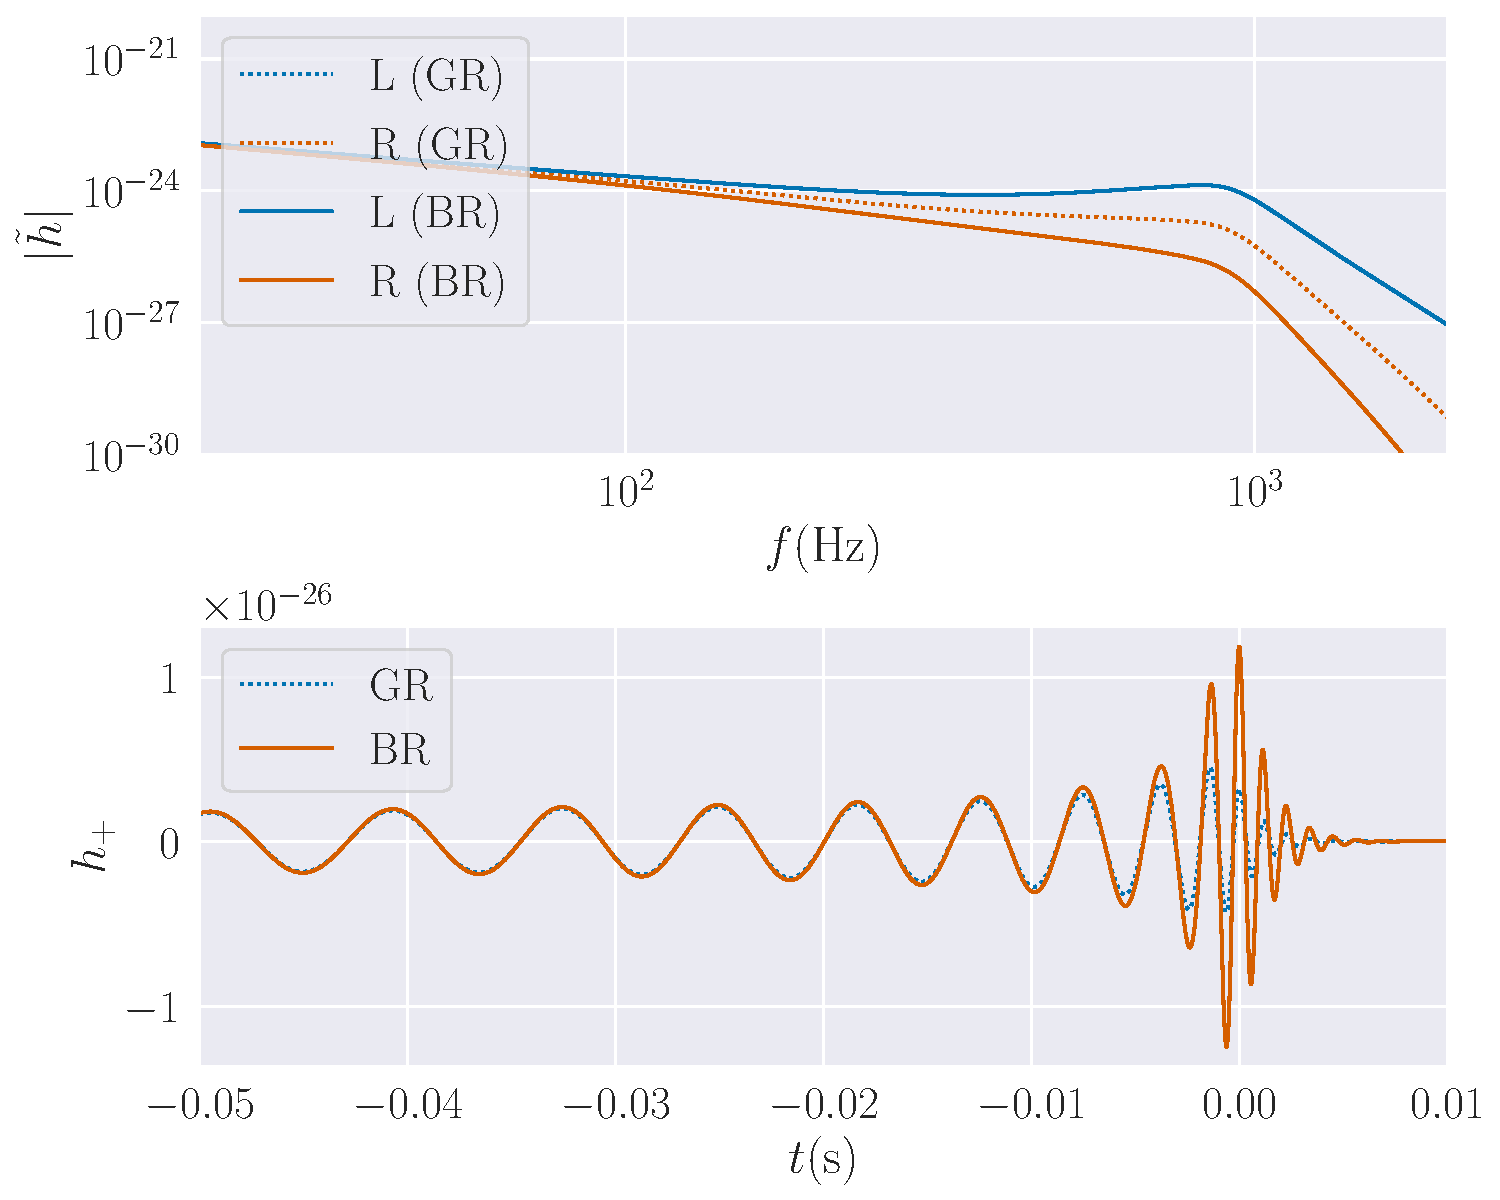
\includegraphics[width=\columnwidth]{figures/birefringence.pdf}
    \caption{
        \emph{Illustration of amplitude birefringence.} The GR waveform for the $\ell=|m|=2$ mode of a nonprecessing BBH seen edge-on ($\cos\iota = 0$) is linearly polarized and thus contains equal amounts of left- and right-handed modes for all frequencies (dotted, top).
        However, if spacetime were birefringent following Eq.~\protect\eqref{eq:waveform_modification}, the waveform observed on Earth would contain different fractions of the two circular modes, with higher frequencies affected more strongly (solid, top). 
        In the time domain, this manifests as a time-dependent amplification of the waveform, with a stronger effect at later times when the chirp reaches a higher instantaneous frequency (bottom).
        For this example, the black holes do not spin and have equal masses $m_1 = m_2 = 10\, M_\odot$, and we have chosen a luminosity distance $d_L = 400\, {\rm Mpc}$ and $\kappa = 0.6$.
        }
    \label{fig:birefringence}
\end{figure}

\citet{Okounkova_2022} took the effect of birefringence to be independent of the frequency, which is a zeroth-order approximation of the birefringence model in Chern-Simons gravity.
This assumption results in a full degeneracy between $\kappa$ and $\iota$:
to reconstruct the amplitude ratio from the interferometer data, an $\iota$ representing a more face-off inspiral can pair with a positive $\kappa$, or an $\iota$ representing a more face-on inspiral with a negative $\kappa$.
That fact can be used to constrain frequency-independent birefringence by searching for features in the distribution of inferred inclinations \cite{Okounkova_2022}.

By implementing Eq.~\eqref{eq:waveform_modification}, which is a first-order approximation of the birefringence model, we generally break the degeneracy between birefringence and source orientation; this was also the case in the frequency-dependent relations studied in \cite{Yamada_2020,Wang_2021}.
Nevertheless, there exist systems for which the degeneracy cannot be perfectly broken because not enough frequencies are available in the data.
As we will see in Sec.~\ref{sec:Results}, this is the case for heavy \acp{BBH}, which are only in the sensitive band of the detectors for a few cycles.

Besides source inclination, the effect of birefringence can be (partially) degenerate with other parameters---most notably, precession, as we find in Sec.~\ref{sec:Results}.
Indeed, under the right conditions, the frequency-dependent amplification/dampening of polarizations caused by $\kappa$ can be effectively absorbed by changes in intrinsic parameters, like the spins;
in that case, the degeneracy with inclination may appear even for lighter \acp{BBH} (although usually to a lesser degree than heavy binaries).
We chart some of these degeneracies as part of the results we present in Sec.~\ref{sec:Results}.
% In particular, we find that, under certain conditions, the frequency-dependent birefringence of Eq.~\eqref{eq:waveform_modification} can mimic the time-dependent amplitude modulation expected from a precessing system.

\section{Method}
\label{sec:Method}

\subsection{Single-event parameter estimation}

To constrain birefringence, we reanalyze events from GWTC-3 \citep{GWTC-2.1, GWTC-3} implementing Eq.~\eqref{eq:waveform_modification} to directly obtain a posterior on $\kappa$ from the strain of each event.
We analyze the 71 \acp{BBH} that were detected with $\mathrm{FAR} < 1/\mathrm{yr}$; to avoid extended computations on longer signals and considering these are generally at closer distances, we do not analyze systems involving neutron stars in this work.
We procure strain data from \ac{GWOSC} \citep{GWOSC}.

We carry out \ac{PE} using a custom version of \textsc{Bilby} \citep{Bilby},
that applies Eq.~\eqref{eq:waveform_modification} for any \ac{GR} baseline
waveform. We take the \ac{PE} configuration as in \citet{GWTC-2.1, GWTC-3,
GWTC-2.1_dataset, GWTC-3_dataset} as a starting point, with
\textsc{IMRPhenomXPHM} \citep{Pratten:2020ceb} as the reference waveform. We
apply a distance prior which is uniform in comoving volume and source frame time, and set the prior on $\kappa$ to a uniform
distribution between $-1$ and $1$. 

For GW190521, we increase the maximum distance of the distance prior to $1.5\times$ the original value, as the birefringence effect enables the probability of a larger distance.
For GW190720, we decrease the analysis segment to 8 s from 16 s, in order to accommodate missing data near the edges of the 16 s segment in Virgo.

In order to validate our \ac{PE} implementation, we reproduce the \ac{LVK} \ac{PE} results obtained assuming \ac{GR} by enforcing $\kappa = 0$; this also has the advantage of producing \ac{GR} runs that are directly comparable to our birefringent runs.
All our \ac{PE} results, including the \ac{GR} validation runs, are published in \citet{dataset}.

\subsection{Collective analysis}

\subsubsection{Shared birefringence parameter}

In the most simplified scenarios, birefringence is a property of spacetime that is not intrinsic to any source or region in space. 
If so, we should expect $\kappa$ to
take the same value for all signals, whether it vanishes or not.
Under this assumption, the
posterior on $\kappa$ inferred collectively from all events 
is simply obtained from the product of the individual likelihoods, $p(d_i \mid
\kappa) \propto p(\kappa \mid d_i)/p(\kappa)$, such that
\begin{equation}
    p(\kappa \mid \{d_i\})\propto p(\kappa) \prod_{i}\frac{p(\kappa \mid d_i)}{p(\kappa)}\,,
    \label{eq:restricted_posterior}
\end{equation}
where $d_i$ is the strain data for the $i$\textsuperscript{th} event, and $p(\kappa)$ is the prior on $\kappa$; since the prior is uniform, in our case Eq.~\eqref{eq:restricted_posterior} reduces to the product of the posteriors, namely $p(\kappa \mid \{d_i\}) \propto \prod_{i}p(\kappa \mid d_i)$.
We use Eq.~\eqref{eq:restricted_posterior} to obtain the primary constraint presented in this work.

\subsubsection{Nonshared birefringence parameters}
\label{sec:method:hier}

% Bayesian Hierarchical Modeling
Under many frameworks, birefringence is brokered by an extra parity-odd
field that couples to gravity. In this case, whether the birefringence
is the same along the different lines of sight to the different events depends
on cosmic history and the local evolution of the field. The \emph{simplest}
assumption is that the field manifests equally for all events, as assumed in the previous subsection, but this is by
no means required.
This motivates a collective analysis that does not assume $\kappa$ is shared across events \cite{Zimmerman:2019wzo,Isi:2022cii}.
Such an analysis has the additional advantage of helping us further characterize our set of measurements, and identify potential outliers.

To do this, we apply hierarchical Bayesian inference \cite{Loredo:2004nn} to model the distribution of $\kappa$'s consistent with the observed data:
we posit that there is a specific value of the parameter, $\kappa_i$, associated with each event, drawn from some unknown distribution of underlying values; from the imperfect measurements of $\kappa_i$ for each event, we may reconstruct the underlying distribution.
If we are interested in constraining the first two moments of the distribution, it is convenient to parametrize the $\kappa_i$'s as drawn from a Gaussian with unknown mean $\mu$ and variance $\sigma^2$, i.e., $\kappa_i \sim \mathcal{N}(\mu, \sigma^2)$ \cite{Isi:2019asy}, and measure those hyperparameters from the collection of observed data.

If \ac{GR} is correct and there is no birefringence, we should find the observed $\kappa$ distribution to be consistent with a delta function at the origin ($\kappa_i = 0$ for all $i$, or $\mu=\sigma=0$); on the other hand, if spacetime is birefringent, we expect to find a delta function at some nonzero value ($\kappa_i = \kappa \neq 0$, or $\mu = \kappa$ and $\sigma=0$).
But this analysis also has the power to reveal unexpected physics or systematics in our measurements: if $\sigma$ is confidently found to be nonzero, this would imply that our set of measurements is statistically unlikely to originate from a unique $\kappa$ value.
This could signal richer physics than is implied by Eq.~\eqref{eq:waveform_modification} or, more prosaically, that there are outliers in our measurements due to mismodeling, e.g., in the waveform approximant or the noise of the detector.

Starting from the posterior on $\kappa$ from each event, the posterior on the hyperparameters $\mu$ and $\sigma$ can be calculated by
\begin{equation}
    p(\mu,\sigma \mid \{d\})\propto p(\mu,\sigma)\prod_{i}\int\frac{p(\kappa_i\mid d_i)}{p(\kappa_i)}p(\kappa_i\mid\mu,\sigma)\,d\kappa_i\,,
    \label{eq:posterior_of_mu_sigma}
\end{equation}
where $p(\kappa)$ is the prior initially applied to $\kappa$ during \ac{PE}, which in our case is a uniform distribution $\mathcal{U}[-1,1]$.
Furhter choosing the hyperpriors on $\mu$ and $\sigma$ to be uniform, Eq.~\eqref{eq:posterior_of_mu_sigma} simplifies to
\begin{equation}
    p(\mu,\sigma\mid\{d\})\propto\prod_{i}\int p(\kappa_i\mid d_i)\mathcal{N}(\mu,\sigma)\,d\kappa_i\,.
\end{equation}

We also calculate the expected population distribution of $\kappa$ marginalized over $\mu$ and $\sigma$.
This is given by
\begin{equation}
            p(\kappa\mid \{d\})=\int \mathcal{N}(\mu,\sigma)p(\mu,\sigma\mid \{d\})\,d\mu\,d\sigma\, , 
    \label{eq:generic_posterior}
\end{equation}
and represents our overall expectation for $\kappa$, given the observed set of individual measurements.
To sample the posterior distribution of $\mu$ and $\sigma$, we use the sampling package \textsc{flowMC} \citep{flowMC}.

\section{Results}
\label{sec:Results}

In this section, we present the results of our study.
We first show the \ac{PE} results of all events and present the results of Bayesian hierarchical modeling.
Then, we will discuss some special events individually.

\begin{figure}
    \script{violin_kappa.py}
    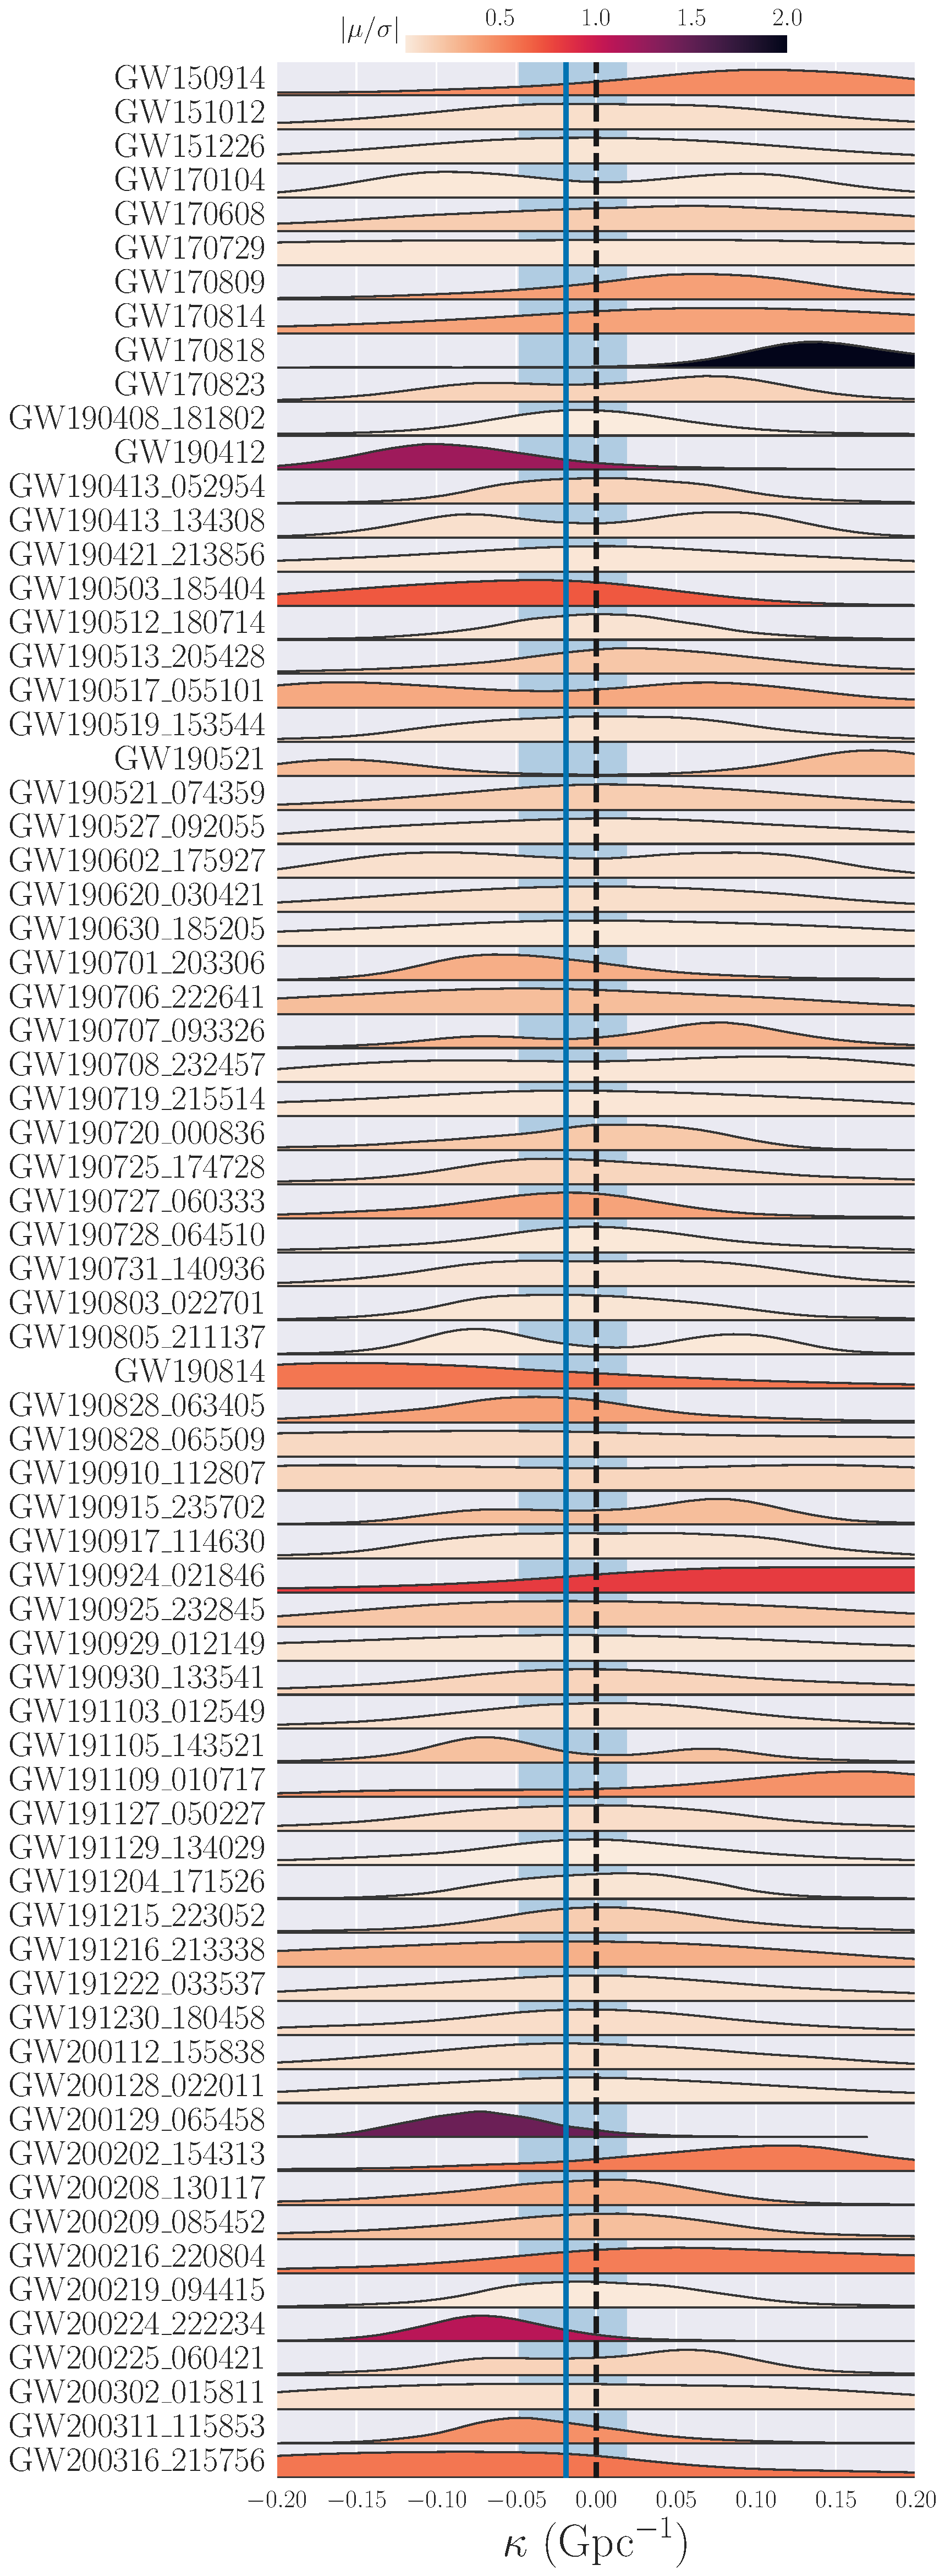
\includegraphics[width=\columnwidth]{figures/violin_kappa.pdf}
    \caption{
        Individual-event $\kappa$ posteriors (distributions), and joint measurement (blue band, 90\% CI; blue line, median).
    }
    \label{fig:violin_kappa}
\end{figure}

\subsection{GWTC-3 result}

% Violin plot
Figure \ref{fig:violin_kappa} shows the main result of our GWTC-3 analysis
as represented by the posterior distribution on $\kappa$ (abscissa) obtained for each event (ordinate). Posteriors are colored by the distance to the origin of the respective mean in units of standard deviation, i.e., $|\mu_i/\sigma_i|$ for each event $i$.%
\footnote{We use the $i$ notation for individual events here to disambiguate from the population mean $\mu$ and standard deviation $\sigma$ of Eq.~\eqref{eq:posterior_of_mu_sigma}.}
The collective measurement obtained by assuming a shared $\kappa$ across events, Eq.~\eqref{eq:restricted_posterior}, is represented by its 90\%-credible symmetric interval (blue band) around the median (blue line);
this joint measurement is fully consistent with $\kappa = 0$ (dashed line), meaning we find no evidence for birefringence.

Figure \ref{fig:violin_kappa} makes it clear that not all \acp{BBH} in GWTC-3 are equally informative about birefringence.
When considered individually, the events that best constrain $\kappa$ are listed in Table~\ref{tab:best_events_kappa}, in order of increasing standard deviation $\sigma_i$.
That table also shows the credible level (CL) at which the posterior supports $\kappa = 0$, whereby $\mathrm{CL} = 0$ ($\mathrm{CL} = 1$) means the posterior supports that value with high (low) probability.

Judging by $\mu_i/\sigma_i$, the two events that show the largest tension with $\kappa = 0$ are GW170818, for which $\mu_i / \sigma_i =$ \variable{output/GW170818_constraint.txt}, and GW200129\_065458 (henceforth GW200129), for which $\mu_i / \sigma_i =$ \variable{output/GW200129_constraint.txt}.
However, as we discuss in Sec.~\ref{sec:GW200129}, we have reason to think that the preference for $\kappa < 0$ in GW200129 might be driven by noise anomalies in the Virgo detector; for that reason, in the next section we consider the effect of excluding this event from the joint result (we find its impact to be minimal).

\begin{table}
    \caption{Events that best constrain $\kappa$, sorted by posterior standard deviation $\sigma_i$. CL is the credible level of $\kappa = 0$.}
    \begin{ruledtabular}
        \variable{output/best_events_kappa.txt}
    \end{ruledtabular}
    \label{tab:best_events_kappa}
\end{table}

\begin{table}
    \caption{Events with bimodality in the $\kappa$ posterior tend to have high total masses. CL is the credible level of $\kappa = 0$.}
    \begin{ruledtabular}
        \variable{output/bimodal_events_mass.txt}
    \end{ruledtabular}
    \label{tab:bimodal_events_mass}
\end{table}

Finally, a set of events stands out in Fig.~\ref{fig:violin_kappa} due to evident bimodality in the $\kappa$ posterior.
To a varying degree, that is the case for those events listed in Table~\ref{tab:bimodal_events_mass}, which tend to have quite high total masses (Table~\ref{tab:bimodal_events_mass} show total mass as measured in the standard  \ac{GR} analysis).
For these bimodal posteriors, $\mu_i/\sigma_i$ is not a good proxy for agreement with \ac{GR}; instead, we can rely on $\mathrm{CL}(\kappa = 0)$.
By this measure, the bimodal events are some of the least consistent with $\kappa = 0$, GW190521 in particular. (However, note that configurations with $\kappa = 0$ for this event are still within the higher dimensional 90\%-credible region, when other parameters are considered and not just the one-dimensional marginal; we discuss this in Sec.~\ref{sec:GW190521}.)

As we mentioned in Sec.~\ref{sec:inclination}, we understand the bimodality in $\kappa$ to be primarily a consequence of the narrow set of frequencies that are visible for these heavy events, which makes the effect of birefringence (partially) degenerate with a change in inclination.
Other parameter degeneracies also come into play, especially for the lighter events GW191105\_143521 (henceforth GW191105) and GW170104.
We discuss this in detail in a dedicated section below (Sec.~\ref{sec:notable}).

\begin{figure}
    \script{corner_Gaussian.py}
    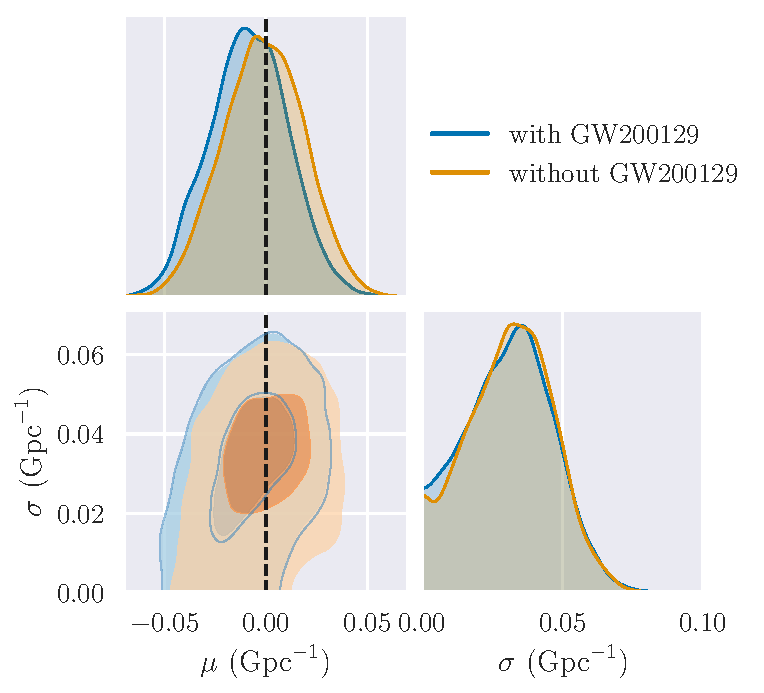
\includegraphics[width=\columnwidth]{figures/corner_Gaussian.pdf}
    \caption{
        The posterior of the $\kappa$ population hyperparameters $\mu$ and $\sigma$, including (blue) and excluding (orange) GW200129 from the collection of events.
        The 2D contours correspond to the $39.35\%$ and $90\%$ credible levels.
        The plot shows that the population constraint on $\kappa$ is consistent with no birefringence ($\mu=\sigma=0$) at the 90\% credible level.
    }
    \label{fig:corner_Gaussian}
\end{figure}

\subsection{Hierarchical modeling}
\label{sec:results:hier}

Figure \ref{fig:violin_kappa} shows certain degree of variance in the distribution of $\kappa$ posteriors for different events, including some apparent outliers like GW170818.
This is not unexpected: assuming independent Gaussian noise instantiations for each event, we might expect up to ${\sim}3$ out of the 71 posteriors (i.e., ${\sim}5\%$) to deviate away from the true $\kappa$ value by over ${\sim}2\sigma$.

To further assess the statistical properties of the set of posteriors in Fig.~\ref{fig:violin_kappa}, we apply the hierarchical analysis described in Sec.~\ref{sec:method:hier}.
By characterizing the population mean and standard deviation over events, this also allows us to obtain a collective measurement that does not assume all events share the same value of $\kappa$.

We summarize the result of this exercise in Fig.~\ref{fig:corner_Gaussian}, which shows the posterior on the population mean $\mu$ and standard deviation $\sigma$ inferred from the collection of observations in Fig.~\ref{fig:violin_kappa}.
The figure shows two distributions, which result from analyses with (blue) and without (orange) the potentially-contaminated event GW200129; the difference between the two is mainly restricted to a slight shift in $\mu$, indicating that GW200129 has a small effect on our overall population inference.

Both versions of the posterior support the lack of birefringence ($\mu = \sigma = 0$) within 90\% credibility; from the marginals of the result including all events, we constrain $\mu =$ \variable{output/mu_median.txt} for 90\%-credible symmetric intervals around the median, and $\sigma <$ \variable{output/sigma_median.txt} for the 90\%-credible one-sided upper limit.
However, even though $\sigma = 0$ is well supported, the $\sigma$ posterior peaks away from the origin, indicating some preference for a nonzero variance.
This could be a sign of the presence of outliers in our sample.

As a check for outliers, we reconsider the set of measurements in Fig.~\ref{fig:violin_kappa} in light of the hierarchical result for $\mu$ and $\sigma$ in Fig.~\ref{fig:corner_Gaussian}, including GW200129 (blue curve).
This amounts to reweighting the $\kappa$ posterior for each event under a population prior marginalized over $\mu$ and $\sigma$, conditional on the measurements from all other events \cite{Callister:T2100301}.
Figure \ref{fig:corner_Gaussian} does not show evidence for any of the events being in obvious tension with the population, even though the GW170818 curve stands out from the rest due to its preference for $\kappa > 0$.
This feature appears to offset a few other events which tend to favor $\kappa < 0$.
The interaction between these distributions leads to a hyperposterior that is fully consistent with $\mu = 0$ while indicating some support for $\sigma > 0$ (Fig.~\ref{fig:corner_Gaussian}).
Future observations will determine whether there is truly evidence for a nonvanishing variance in this population.

\begin{figure}
    \script{reweighed_kappa.py}
    \includegraphics[width=\columnwidth]{figures/reweighed_kappa.pdf}
    \caption{Individual-event $\kappa_i$ distributions of Fig.~\ref{fig:violin_kappa} reweighted in light of the population-level inference of Fig.~\ref{fig:corner_Gaussian}, marginalizing over $\mu$ and $\sigma$. Curves are colored by the magnitude of the supported deviation, as represented by the respective posterior $|\mu_i / \sigma_i$; we label the events most in tension with $\kappa_i = 0$ by that same measure.}
    \label{fig:reweighted_kappa}
\end{figure}

% Constraint on $\kappa$
Finally, the hierarchical result in Fig.~\ref{fig:corner_Gaussian} can be translated into an overall expectation for $\kappa_i$ via Eq.~\eqref{eq:generic_posterior}.
We show the result of doing this in Fig.~\ref{fig:posterior_kappa}, where we also compare to the posterior on $\kappa$ obtained by assuming a shared value across events (same result shown as a blue band in Fig.~\ref{fig:violin_kappa}).
The hierarchical measurement leads to an expectation that $\kappa_i = $\variable{output/generic_kappa_median.txt}, whereas the shared-$\kappa$ measurement implies $\kappa = $\variable{output/restricted_kappa_median.txt}, both symmetric 90\%-credible intervals around the median.  

\begin{figure}
    \script{posterior_kappa.py}
    \includegraphics[width=\columnwidth]{figures/posterior_kappa.pdf}
    \caption{
        The generic and restricted posterior of $\kappa$.
        The blue solid and dashed lines show the restricted posterior of $\kappa$ with and without GW200129, respectively.
        The orange solid and dashed lines show the generic posterior of $\kappa$ with and without GW200129, respectively.
        The black dashed line marks the absence of birefringence ($\kappa=0$).
    }
    \label{fig:posterior_kappa}
\end{figure}

% Case studies
\subsection{Notable events}
\label{sec:notable}

Having established that the collection of detections is globally consistent with $\kappa=0$, here we focus on four events whose $\kappa$ posteriors stand out in Fig.~\ref{fig:posterior_kappa}: GW170818, GW200129, GW190521 and GW191105\_143521.

When considered in isolation, the first of these is the event with the most significant support for nonzero $\kappa$; the second shows the sign of potential noise anomalies; the third is representative of a class of heavy events with strongly bimodal $\kappa$ posteriors; and the fourth of a small class of lighter events with slightly bimodal posteriors.

% Case: GW170818
\subsubsection{GW170818}
\label{sec:GW170818}

GW170818 produced the posterior in most tension with $\kappa=0$, when judged by $\mu_i/\sigma_i$ in Fig.~\ref{fig:violin_kappa}.
Figure \ref{fig:corner_GW170818} shows that this happens because birefringence opens up a region of parameter space with $\kappa>0$ for larger distances and smaller inclination angles than would be allowed in the GR case.
We can make sense of this because an edge-on, nonprecessing source will produce linearly-polarized waves, so a smaller inclination will lead the two circular polarizations to have similar amplitudes.
On the other hand, having $\kappa > 0$ will enhance the left-handed modes during propagation.
The two effects can be balanced to yield the correct polarization ratio at the detector, as long as the distance is also enhanced to yield the right amount of birefringence and overall signal power.
This is similar to the degeneracy mentioned in Sec.~\ref{sec:inclination}.
% Even though the degeneracy is broken by the frequency dependence to a large extent, it is still possible for getting an extra region with a nonzero $\kappa$.
% This is because there is still a significant likelihood in the region of $\kappa$ close to zero.
% We can see this effect in other events as well, but not as strongly as in GW170818.

It is not clear what specific feature of the GW170818 data leads to this posterior structure.
However, the reason may be related to the fact that this event provides an uncommonly definite measurement of the polarization angle and spin orientations \cite{Varma:2021csh}.
Indeed, the inferred polarization angle and spins in the birefringent case are notably different from the \ac{GR} case (Fig.~\ref{fig:corner_GW170818_appendix}).
If our inference on $\kappa$ is indeed tied to those parameters, we might be susceptible to systematics in the modeling of spin angles in \textsc{IMRPhenomXPHM} and might thus benefit from further analysis with other waveforms like \textsc{NRSur7dq4} \cite{Varma:2018mmi}.
In any case, as we argued in Sec.~\ref{sec:results:hier}, there is no evidence at the moment that this event is inconsistent with the either collection of measurements or with $\kappa = 0$ (Fig.~\ref{fig:reweighted_kappa}).

\begin{figure}
    \script{corner_GW170818.py}
    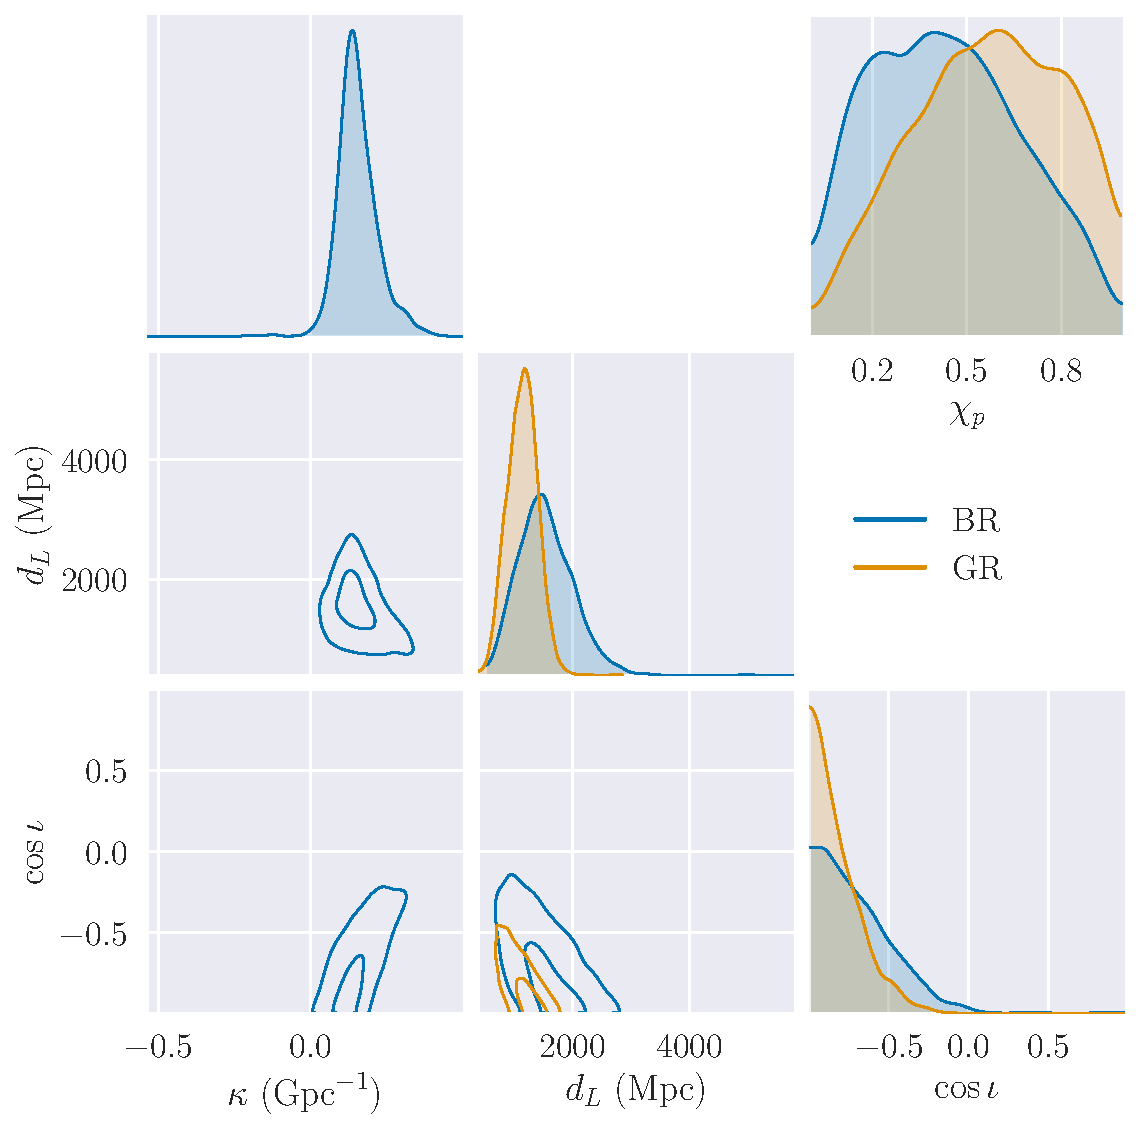
\includegraphics[width=\columnwidth]{figures/corner_GW170818.pdf}
    \caption{GW170818 posterior on $\kappa$, luminosity distance $d_L$ and inclination $\cos\iota$ from our birefringence analysis (blue), compared to the GR result (orange).}
    \label{fig:corner_GW170818}
\end{figure}

% Case: GW200129 (glitch in Virgo data)
\subsubsection{GW200129}
\label{sec:GW200129}

GW200129 is the event with the second largest $|\mu_i/\sigma_i|$ in Fig.~\ref{fig:violin_kappa}.
However, data for this event were affected by a non-Gaussian noise disturbance (glitch) in the Virgo instrument, which was subtracted from the publicly-available data used for parameter estimation \cite{Davis:2022ird}.
Since previous work suggests the degree of glitch subtraction affects the inference for this event \citep{GW200129_glitch}, we consider whether the apparent preference for $\kappa < 0$ could also be tied to the instrumental artifact.

To this end, we perform three additional \ac{PE} runs for GW200129, considering only two detectors at a time: LIGO Hanford and Virgo (HL), LIGO Livingston and Virgo (LV), and LIGO Hanford and LIGO Livingston (HL).
If the preference for $\kappa < 0$ is tied to the glitch in Virgo, we expect it to disappear in the HL run, which excludes Virgo data.

This is indeed the case, as we show in Fig.~\ref{fig:corner_GW200129}: all runs including Virgo lean towards $\kappa < 0$ (solid curves in color), whereas the LIGO-only run is fully consistent with $\kappa = 0$ (dashed black).
While this is not conclusive proof that the glitch itself is driving the result, it does indicate that the Virgo data play a key role in the inference of $\kappa$.
Since more work would be needed to understand the effect of the glitch, this motivates us to consider the effect of excluding this event from the collective analyses above.

\begin{figure}
    \script{corner_GW200129.py}
    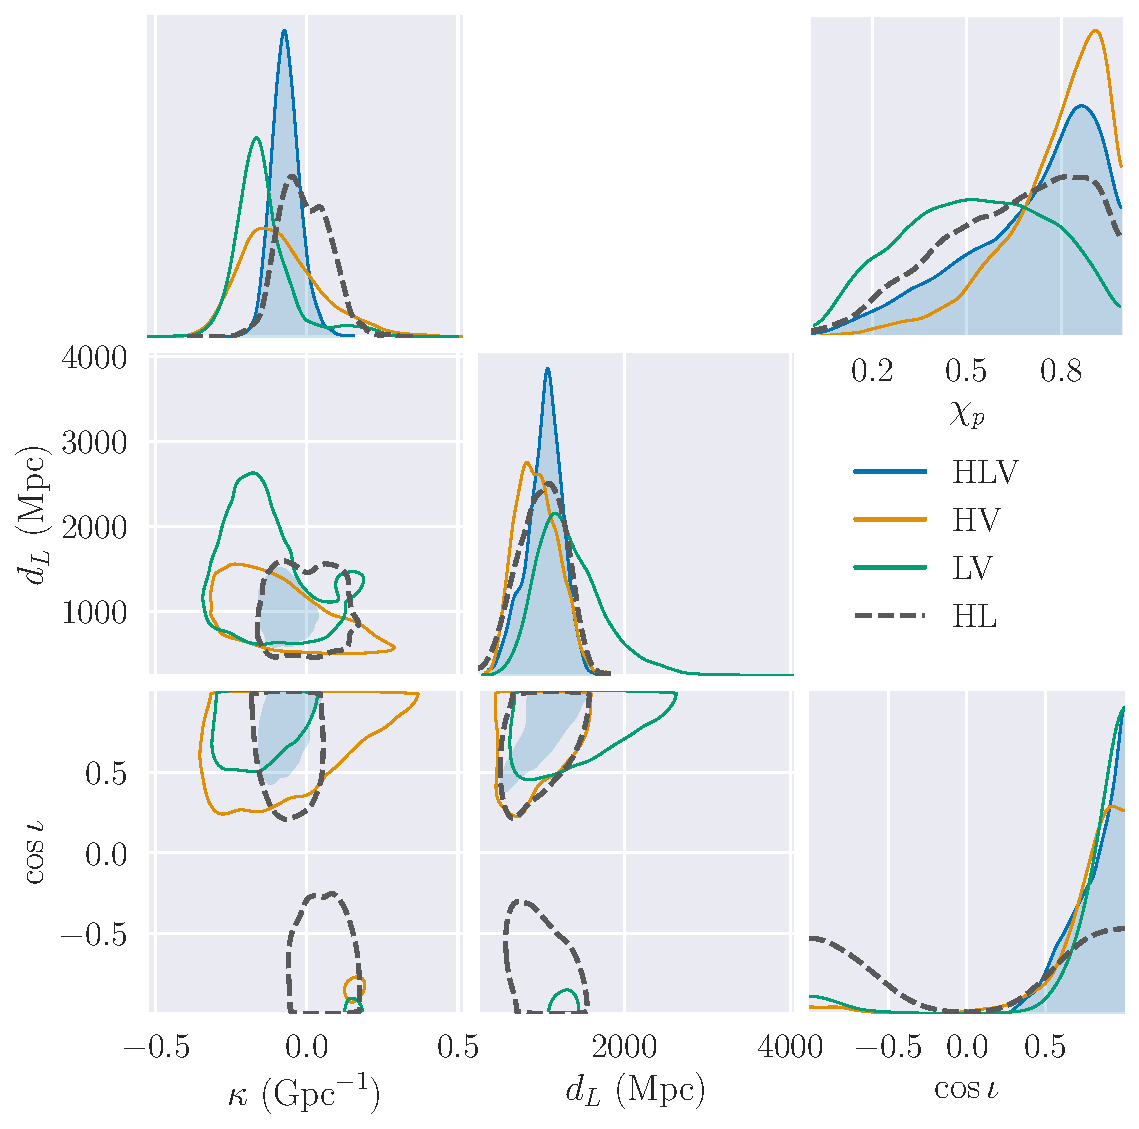
\includegraphics[width=\columnwidth]{figures/corner_GW200129.pdf}
    \caption{
        GW200129 posterior on $\kappa$, luminosity distance $d_L$ and inclination $\cos{\iota}$, including different sets of detectors in the analysis per the legend.
        The main run with all three detectors (HLV, filled blue), shows a preference for $\kappa < 0$, as in Fig.~\ref{fig:violin_kappa}; this preference is more pronounced for two-detector runs that include Virgo (HV and LV, orange and green); however, it disappears if we remove Virgo (HL, dashed black).
        The 2D contours correspond to the $90\%$ credible level.
    }
    \label{fig:corner_GW200129}
\end{figure}

% Case: GW190521 (massive BBH)
\subsubsection{GW190521}
\label{sec:GW190521}

Even with the frequency-dependent birefringence model, some events still have a bimodal $\kappa$ distribution.
Consider GW190521, the most massive binary black hole merger in the events we included.
The degeneracy between $\kappa$ and $\iota$ cannot be broken by the frequency-dependent birefringence model, as shown in Fig.~\ref{fig:corner_GW190521}.
The reason could be this GW event's frequency range is too narrow to break the degeneracy.
The effect of birefringence at different frequencies within the range is similar, so the degeneracy cannot be broken.
Therefore, the narrow frequency range can be a possible reason why the $\kappa$ distribution of GW190521 is bimodal.
Note that $\kappa=0$ is still within the $90\%$ confidence interval, with a non-negligible probability.
The bimodal $\kappa$ distribution only means that the degeneracy between $\kappa$ and $\iota$ cannot be broken in this case.  \wf{You should still explain \emph{why} the model seems to prefer $\left| \kappa \right| > 0$.  I \emph{think} the reason here is the distance prior---there is a lot more ``phase space'' at large distances that can be accessed by allowing $\kappa$ to be non-zero and choosing a corresponding inclination so that the amplification effects of birefringence are compensated for by the larger distance compared to the pure-GR run.  Does this make sense to you?  If so, can you write it up in this paragraph?}

\begin{figure}[h]
    \script{corner_GW190521.py}
    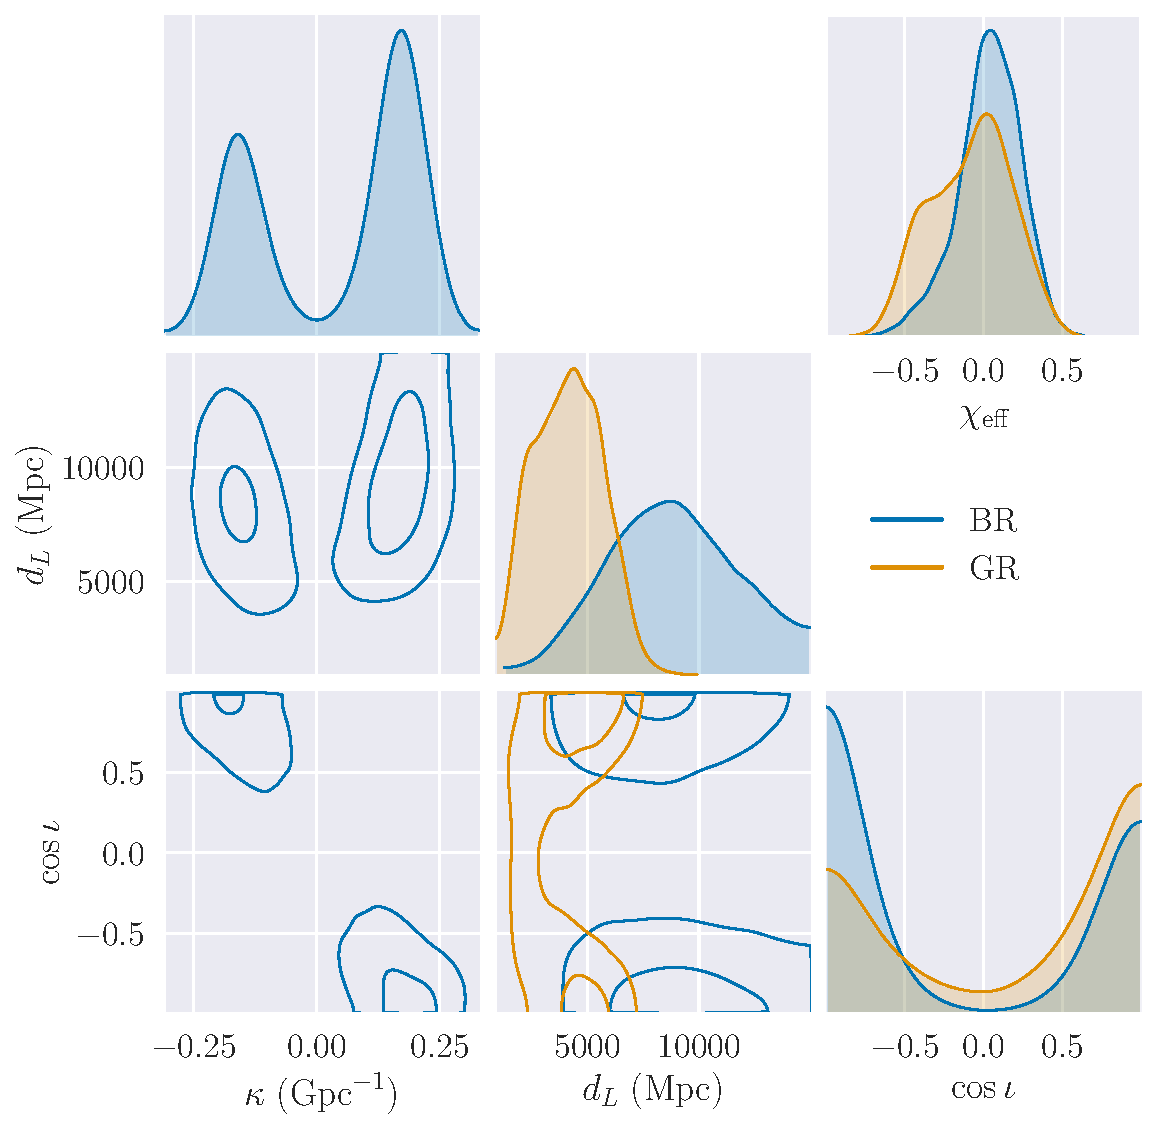
\includegraphics[width=\columnwidth]{figures/corner_GW190521.pdf}
    \caption{
        GW190521 posterior on $\kappa$, luminosity distance $d_L$ and inclination $\cos\iota$ from our birefringence analysis (blue), compared to the GR result (orange).
        % The posterior of $\kappa$, luminosity distance $d_L$ and $\cos{\iota}$ for GW190521.
        % Colors in the plot represent the \ac{PE} result with \ac{GR} and the frequency-dependent birefringence, respectively.
        % The 2D contours correspond to the $39.35\%$ ($1\sigma$) and $90\%$ credible levels.
        % This plot shows that frequency-dependent birefringence cannot break the degeneracy between $\kappa$ and $\iota$.
    }
    \label{fig:corner_GW190521}
\end{figure}

% Case: GW150914 (example of broken degeneracy)
\subsubsection{GW150914}
In this study, we included frequency dependence of birefringence, which would affect the posterior of $\kappa$ obtained from \ac{PE}.
Consider GW150914, the first GW detected by LIGO, as an example.
In Fig.~\ref{fig:corner_GW150914}, we show the posteriors of the parameters of GW150914.
With the frequency-independent birefringence model, the posteriors for $\cos\iota$ look different from the posteriors assuming GR.
This is because, for a nonprecessing system, there is a degeneracy between $\kappa$ and $\iota$ if the frequency dependence is not included.
% explain the kappa gap

On the other hand, with the frequency-dependent birefringence model, the posterior looks similar to the GR posterior.
This is because the frequency dependence broke the degeneracy, as the effect of birefringence will differ from the effect of changing $\iota$.
In this case, the most probable value of $\kappa$ is close to $0$, which means the birefringence is weak or absent.
Therefore, the \ac{PE} result with frequency dependence is consistent with GR.

\begin{figure}
    \script{corner_GW150914.py}
    \includegraphics[width=\columnwidth]{figures/corner_GW150914.pdf}
    \caption{
        GW150914 posterior on $\kappa$, luminosity distance $d_L$ and inclination $\cos\iota$ from our frequency-dependent (blue) and frequency-independent (orange) birefringence analysis, compared to the GR result (green).
        % The posterior of $\kappa$, luminosity distance $d_L$ and $\cos{\iota}$ for GW150914.
        % Colors in the plot represent the \ac{PE} result with \ac{GR}, frequency-independent and dependent birefringence, respectively.
        % The 2D contours correspond to the $39.35\%$ ($1\sigma$) and $90\%$ credible levels.
        % Note that there is no posterior of $\kappa$ for the \ac{PE} result with \ac{GR}, as the result is based on GR, which does not suggest GW amplitude birefringence.
        % This plot shows that frequency-independent birefringence creates a degeneracy between $\kappa$ and $\iota$, while frequency-dependent birefringence can break it.
    }
    \label{fig:corner_GW150914}
\end{figure}

\section{Discussion}
\label{sec:Discussion}

% Comparison with previous studies
\subsection{Comparison with previous studies}
\citet{Okounkova_2022} gave a constraint on GW amplitude birefringence by performing statistical analysis on GWTC-2.
We convert the constraint they gave to the same units as ours to make a comparison.
They were able to constrain $\kappa$ to be $|\kappa| \lesssim 0.74$ at $1 \sigma$.
We obtained a tighter constraint on $\kappa$ with $|\kappa| \lesssim 0.04$ at $1 \sigma$.
Our result is an order of magnitude improvement in constraining $\kappa$.
The main reason is that we have more events from GWTC-3 than GWTC-2.

\citet{Wang_2021} performed \ac{PE} on GWTC-1 events with a frequency-dependent birefringence model.
They formulated the birefringence effect as corrections to the GW waveform on a linear basis.
We convert their constraint to the same units as ours with the derivation in Appendix~\ref{sec:M_PV_derivation}.  \wf{Can you give the answer here (as well as in Appendix B)?}
% Discussion on the difference between our work and theirs

% Future work
\subsection{Future work}
% BNS
Future work is to perform \ac{PE} on binary neutron star mergers, such as GW170817.
The frequency range of the signal is much wider compared to the binary black hole mergers.
Thus, the difference in the effect of birefringence at different frequencies within the range can be more significant.
The \ac{PE} on binary neutron star mergers can allow us to further constrain the birefringence effect and the beyond-GR theories that predict it.
However, performing \ac{PE} on binary neutron star mergers requires much more computational resources.
Therefore, we may need to wait for future \ac{PE} methods and tools to further our work.

% More observations with higher SNR
Another future work is to apply the same method to more GW events and events with a higher signal-to-noise ratio (SNR).
LVK will release more events with higher SNR in the future.
Using data with higher SNR allows us to obtain more precise \ac{PE} results and constrain the birefringence effect more precisely.
And using data from more events will allow us to calculate a more constrained population posterior of $\kappa$.

\begin{acknowledgments}
M.~I., K.~W.~K.~W.~, and W.~M.~F.~ are funded by the Center for Computational Astrophysics at the Flatiron Institute.
The Flatiron Institute provided the computational resources used in this work.

This research has made use of data or software obtained from the Gravitational Wave Open Science Center (gwosc.org), a service of LIGO Laboratory, the LIGO Scientific Collaboration, the Virgo Collaboration, and KAGRA.
LIGO Laboratory and Advanced LIGO are funded by the United States National Science Foundation (NSF) as well as the Science and Technology Facilities Council (STFC) of the United Kingdom, the Max-Planck-Society (MPS), and the State of Niedersachsen/Germany for support of the construction of Advanced LIGO and construction and operation of the GEO600 detector.
Additional support for Advanced LIGO was provided by the Australian Research Council.
Virgo is funded, through the European Gravitational Observatory (EGO), by the French Centre National de Recherche Scientifique (CNRS), the Italian Istituto Nazionale di Fisica Nucleare (INFN) and the Dutch Nikhef, with contributions by institutions from Belgium, Germany, Greece, Hungary, Ireland, Japan, Monaco, Poland, Portugal, Spain.
KAGRA is supported by Ministry of Education, Culture, Sports, Science and Technology (MEXT), Japan Society for the Promotion of Science (JSPS) in Japan; National Research Foundation (NRF) and Ministry of Science and ICT (MSIT) in Korea; Academia Sinica (AS) and National Science and Technology Council (NSTC) in Taiwan.
\end{acknowledgments}

\appendix

\section{placeholder for GW191105}

\begin{figure}[h]
    \script{corner_GW191105.py}
    \includegraphics[width=\columnwidth]{figures/corner_GW191105.pdf}
    \caption{
        Corner plot of GW191105.
    }
    \label{fig:corner_GW191105}
\end{figure}

\section{GW170818}

\begin{figure*}[h]
    \script{corner_GW170818_appendix.py}
    \includegraphics[width=\textwidth]{figures/corner_GW170818_appendix.pdf}
    \caption{
        Corner plot of GW170818.
    }
    \label{fig:corner_GW170818_appendix}
\end{figure*}

\begin{figure}
    \script{hist_GW170818.py}
    \includegraphics[width=\columnwidth]{figures/hist_GW170818.pdf}
    \caption{
        Corner plot of GW170818.
    }
    \label{fig:hist_GW170818}
\end{figure}

\section{Relation between $\kappa$ and $M_{PV}$}
\label{sec:M_PV_derivation}

\citet{Wang_2021} formulated the birefringence effect as
\begin{equation}
    h_{+/\times}^{PV}(f) = h_{+/\times}^{GR}(f)\mp h_{\times/+}^{GR}(f)(i\delta h-\delta\Psi)\,,
\end{equation}
where $h_{+/\times}^{PV}(f)$ is the modified \ac{GW} waveform in the linear basis, $h_{+/\times}^{GR}(f)$ is the \ac{GW} waveform in the linear basis as \ac{GR} predicts, $\delta h$ is the amplitude modification, and $\delta\Psi$ is the phase modification.
We can rewrite the equation as
\begin{equation}
\begin{split}
    h_{L/R}^{PV}(f)&=h_{L/R}^{GR}(f)(1\mp\delta h\mp i\delta\Psi)\\
    &\approx h_{L/R}^{GR}(f)\exp\left(\mp\delta h\mp i\delta\Psi\right)
\end{split}
\,,
\end{equation}
where $h_{L/R}^{PV}(f)$ is the modified \ac{GW} waveform in the circular basis, $h_{L/R}^{GR}(f)$ is the \ac{GW} waveform in the circular basis as \ac{GR} predicts.
This equation applies to any birefringence model that allows the assumption that the modification to \ac{GR} is small when observed very near the source.
To make a comparison with our work, we can choose $\delta\Psi=0$, which is a case that \citet{Wang_2021} considered.
In their work, they parametrized $\delta h=-A_\nu\pi f$, while
\begin{equation}
    A_\nu=M_{PV}^{-1}(\alpha_\nu(z=0)-\alpha_\nu(z)(1+z))\,,
\end{equation}
where $A_\nu$ is the parity-violating parameter for amplitude birefringence, $M_{PV}$ is the characteristic energy scale, and $\alpha_\nu$ is a arbitrary functions determined by the birefringence model.
They then chose $\alpha_\nu=1$.
Therefore, we can rewrite the equation as
\begin{equation}
    h_{L/R}^{PV}(f)= h_{L/R}^{GR}(f)\exp\left(\mp\frac{\pi zf}{M_{PV}}\right)\,.
\end{equation}
This equation takes the same form as Eq.~\eqref{eq:waveform_modification}.
We can then find the relation between $M_{PV}$ and $\kappa$ by
\begin{equation}
    \left|\mp\frac{\pi zf}{M_{PV}}\right|=\left|\pm\kappa\frac{d_C}{1\,\mathrm{Gpc}}\frac{f}{100\,\mathrm{Hz}}\right|\,.
\end{equation}
Using $H_0d_C=cz$, where $H_0$ is the Hubble constant and $c$ is the speed of light, we can rewrite the equation as
\begin{equation}
    \kappa=\frac{\pi H_0}{c}\left(1\,\mathrm{Gpc}\right)\left(100\,\mathrm{Hz}\right)M_{PV}^{-1}\,.
\end{equation}

\bibliography{bib}

\end{document}
